\documentclass[11pt,letterpaper]{article}

\usepackage{RPK550_R_Syllabus}

\begin{document}

\begin{center} 
 {\titlefont
		
		\Huge
		\textbf{SMEA 500:}
		
		Coding in \R for Natural and Social Sciences
}

\large
Fall 2018
	
Wednesdays 12:30pm -- 2:20pm

OUG 141

{\titlefont
		Ryan Kelly \& Ramón Gallego\\
		Office Hours: By appointment\\
		\Letter\ \href{mailto:rpkelly@uw.edu}{rpkelly@uw.edu} ; \href{mailto:rgallego@uw.edu}{rgallego@uw.edu}		
}

\end{center}
\setlength{\parskip}{1em}


\begin{figure}[!ht]
\begin{center}
  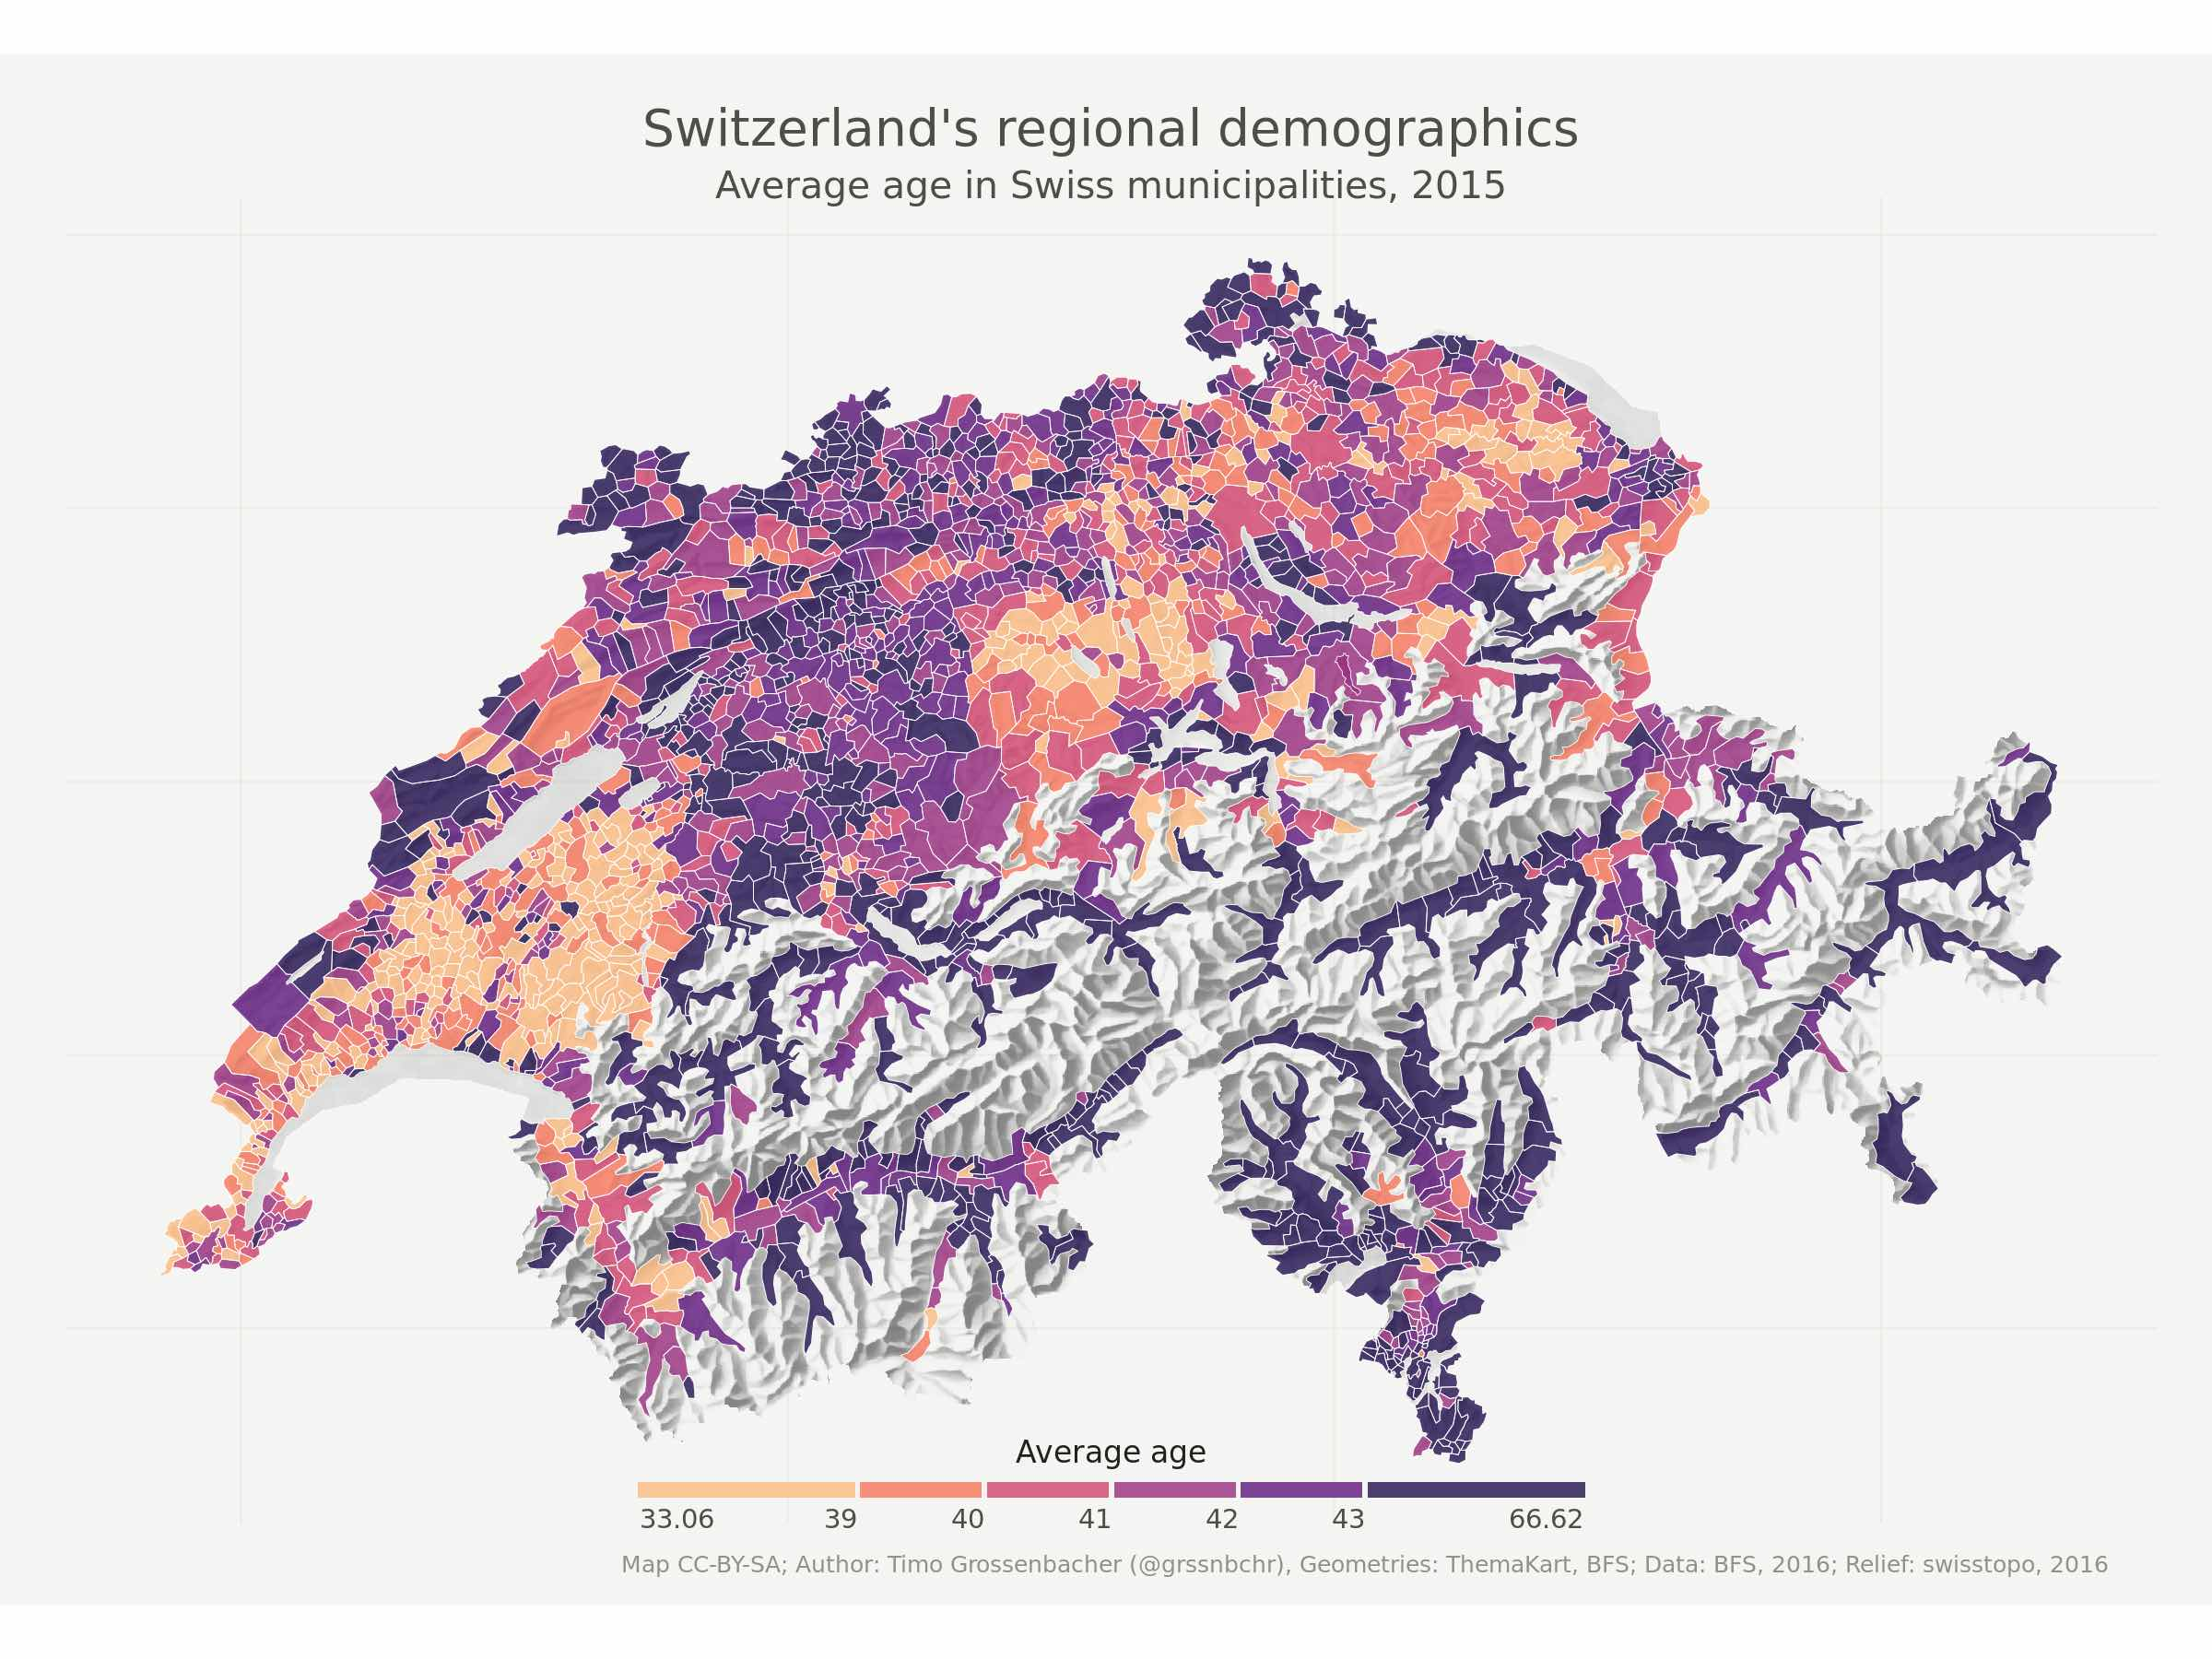
\includegraphics[width = 0.7\textwidth]{tm-final-map-1.jpg}
\end{center}
\end{figure}



Some degree of computer coding is increasingly a required skill for all kinds of careers. As natural and social scientists, we often have to analyze large datasets or undertake repetitive analytical tasks that do not lend themselves well to working with spreadsheets. We generally would also like to create powerful graphics that clearly express the conclusions we reach. The free, open-source statistical coding language \R has become a common way for academics and others to tackle these challenges. This course will provide an introduction to \R and give students the tools to become autonomous users if they so desire. Each week will feature a topical presentation, followed by workshop time during which students can troubleshoot and practice their skills on work of their own choosing (e.g., stats problem sets, thesis analyses, or graphics for capstones). No prior coding experience is required, but an open and exploratory mindset will be essential. 

\vspace{1em}

{\Large Learning Goals}\hrulefill
\begin{quote} %using quote here and throughout as a quick way to do paragraph indentation

1) to become familiar with fundamentals of \R

2) to become a more productive and efficient user of data

3) to overcome any fear of computer coding that may be lingering in your mind

4) to do work you already have to do, but do it better
\end{quote}
{\Large Format}\hrulefill

We will spend the first half of each class session in lecture, and the half in workshop to practice the newly acquired skills (or to do your homework).  You should bring a laptop to class with you, with a version of \R running. If you do not have a laptop, you can borrow one from SMEA or from the library.  All books/materials/etc. will be provided, also for free. 

{\Large Book}\hrulefill

We weren't planning to use a book for this class, but it turns out there's a great one that's free and fun.  It's \textit{YaRrr! The Pirate's Guide to \R}.  You can download both the book and the source code used in the book \href{https://ndphillips.github.io/piratesguide.html}{\underline{here}}.  It's by a guy named Nathaniel Phillips, and it would make a good deal of sense to send him some money to support his good work. He has a paypal link on the page where you get the book/code. 

{\Large Grading}\hrulefill

This class is Pass/Fail. You will Pass as long as you show up and try. You may be asked to drop for more than one unexcused absence, or for violations of the College's code of academic conduct (see below).


{\Large How Do I Get and Install \R?}\hrulefill

There are choices.
\begin{itemize}
	\item  Most people like to use \textsf{RStudio}, which is a fully-integrated development environment (that is, it's pretty, and has all kinds of useful functions).  To get that, go here: \url{https://www.rstudio.com/products/RStudio/#Desktop}, and download/install the free version, according to the instructions. For this class, just use this one, so that everyone is on the same page. 
	\item For the record: those of you who want a more stripped-down, customizable version can use plain old \R. Go here: \url{https://cran.r-project.org/}. Follow the instructions. 
	\item For those of you who want to fully live in the Matrix,  and use \R only at the command-line, you probably aren't taking this class.  But there are instructions for this \href{https://cran.r-project.org/doc/manuals/r-patched/R-admin.html#Getting-and-unpacking-the-sources}{\underline{here}}.

\end{itemize}

\R has a large and vibrant community of users, contributors, and supporters. We will soon see that many of the functions of \R come from users themselves, who contribute code to the overall project. You then download and install these contributed functions (called ``packages''), extending the base-\R that you got when you first downloaded it. In this way, \R is a community-wide project that is always expanding. 

And this means that if you have a question, Google it.  You will find answers to nearly every question on one of a few sites, such as \url{https://stackoverflow.com}.

{\Large Computers, Phones, etc.}\hrulefill

Normally we effectively ban laptops from our classes, but for this class they're indispensable, obviously. So we do ask that you use them with due respect for the class and for your classmates. Please do not be buying shoes, using Facebook, or talking on the phone in class.

{\Large Academic Integrity}\hrulefill

You are responsible for understanding the College of the Environment's
rules on academic misconduct. See
\url{http://coenv.washington.edu/intranet/academics/academic-policies/academic-misconduct/}.

Note that it's not obvious what constitutes plagiarism in the case of computer coding (see \href{https://www.nytimes.com/2017/05/29/us/computer-science-cheating.html}{\underline{this article}}). But for our purposes, can we just agree that you're going to do your own work? Certainly, copying code from others is often an accepted part of computer coding -- particularly in an open-source environment -- but there is a difference between using 2 lines of code and using a whole assignment.
\pagebreak

\huge Schedule
\hrulefill

\normalsize


\textbf{\textsc{Week 1}}
		\begin{quote}	
		September 26 \textbullet \space Introduction to the course and to \R. Objects, functions, and getting to be a bit more comfortable with \R.
		
		\textbf{Reading}: \textit{Pirate's Guide} Chapters 1 and 2. 
		Always remember that clear thinking leads to sensible analysis, rather than the other way around.
		
		\textbf{Assigned: Problem Set 1.  Due October 9.}
		
		\end{quote}

\textbf{\textsc{Week 2}}
		\begin{quote}	
		October 3  \textbullet \space Basic computation and stats, and getting data into (and out of) \R. 
		
		\textbf{Reading}: \textit{Pirate's Guide} Chapters 5 and 9.	
		\end{quote}

\textbf{\textsc{Week 3}}
		\begin{quote}	
		October 10  \textbullet \space Plotting 1 (base \R). 
		
		\textbf{Reading}: \textit{Pirate's Guide} Chapter 11

		\textbf{Assigned: Problem Set 2.  Due October 23.}

		\end{quote}

\textbf{\textsc{Week 4}}
		\begin{quote}	
		October 17  \textbullet \space Data Cleaning and Management. 
		
		\textbf{Reading}: \textit{Pirate's Guide} Skim/Review Chapter 9.
		\end{quote}


\textbf{\textsc{Week 5}}
		\begin{quote}	
		October 24  \textbullet \space Loops and other ways to iterate. 
		
		\textbf{Reading}: \textit{Pirate's Guide} Chapter 17.

		\textbf{Assigned: Problem Set 3.  Due November 6.}

		\end{quote}

\textbf{\textsc{Week 6}}
		\begin{quote}	
		October 31  \textbullet \space Testing Hypotheses. 
		
		\textbf{Reading}: \textit{Pirate's Guide} Chapter 13.
		\end{quote}


\textbf{\textsc{Week 7}}
		\begin{quote}	
		November 7  \textbullet \space Plotting 2 (ggplot). 
		
		\textbf{Reading}: Introduction chapter of ggplot2 (book), by Hadley Wickham.  And this \href{http://r-statistics.co/Complete-Ggplot2-Tutorial-Part1-With-R-Code.html}{\underline{tutorial}} is pretty useful.

		\textbf{Assigned: Problem Set 4.  Due December 4.}

		\end{quote}

\textbf{\textsc{Week 8}}
		\begin{quote}	
		November 14  \textbullet \space Dipping a toe into the Tidyverse. 
		
		\textbf{Reading}: David Robinson, ``Teach the Tidyverse to Beginners''
		\end{quote}

\textbf{\textsc{Week 9}}
		\begin{quote}	
		November 21  \textbullet \space Aggregation and Grouping 
		
		\textbf{Reading}: None
		\end{quote}

\textbf{\textsc{Week 10}}
		\begin{quote}	
		November 28 \textbullet \space Tidyverse 2
		
		\textbf{Reading}:  Skim ggplot2 book for useful nuggets.
		\end{quote}

\textbf{\textsc{Week 11}}
		\begin{quote}	
		December  5 \textbullet \space Project Management and Workflow: putting everything together from setup to cleaning, importing, calculating, testing, plotting, and presenting. 
		
		\textbf{Reading}:  None 
		\end{quote}



\vfill
{\tiny Nerdery: typeset in Raleway Light, with title in Archer}

\end{document}
